\chapter{Bayesian learning for DPPs}

So far we have seen two different estimation techniques for the parameters of DPPs. Although we proved that they provide reasonable estimators in the sense that they are consistent, they have some drawbacks. For example we have seen that the MLEs for the different parameters do not exist in general, let alone that they are impossible to compute in reality. Further
%Firstly, we saw that the maximum likelihood estimator does not exist in general and in some cases one needs a fairly high amount of samples to ensure that it does. Secondly 
all of the estimators presented so far are point estimators, i.e. they return a single value for the desired parameter. Obviously this does not allow to capture any uncertainties and we have already seen in \todo{cite} that the selection of the most possible outcome -- in this case the MLE -- might not yield a very typical one for a given random variable.
Those are some reasons to consider the Bayesian approach of parameter estimation where the goal is to give a distribution -- called the posterior -- of the parameter that should be estimated instead of a single value. This can also help to overcome some -- maybe even all of the problems presented above.

At first we will present the general idea of Bayesian parameter estimation and then we will turn towards the question of computability. %Since the normalisation constant of the 
For this we will follow the approach of \cite{affandi2014learning} and turn towards the popular Markov chain Monte Carlo (MCMC) methods and quickly explain their philosophy and how they can be used to approximate the posterior distribution of the parameter that is to be estimated.

\section{Bayesian approach to parameter estimation}

For the introduction of the general Bayesian setup we pursue like in \cite{rice2006mathematical}. We are -- just like in the case of MLE -- in the setting that we want to estimate a parameter \(\theta\in\Theta\) based on some relisations \(x = (x_1, \dots, x_n)\) of some random variables \(X = (X_1, \dots, X_n)\) where we have given a family
\[\mathcal F = \Big\{ f_{X| \Theta}(\cdot |\theta) \mid \theta\in\Theta\Big\}\]
of densities with respect to \(\mu^n\coloneqq\prod_{i=1}^n\mu(\mathrm d x_i)\). This time however we are not interested in returning a single value \(\theta\) because this would be a vast simplification of the stochastic nature of the estimator. Thus we want to obtain a probability distribution over whole \(\Theta\) that indicates how the parameters are to have caused the observed data. In order to present the procedure we will introduce the frame we will work in.

\begin{emp}[Setting]
Let \(\Theta\) be a measurable space and \(\nu\) be a measure on \(\Theta\). Further let \(f_\Theta\colon \Theta\to[0, \infty]\) be a probability density with respect to \(\nu\), i.e.
\[\int f_\Theta(\theta)\nu(\mathrm{d}\theta) = 1\]
which we will call the \emph{prior} distribution of the parameter \(\theta\).
\end{emp}

Usually the prior distribution will encode some perceptions we have of the parameter. For example if we are trying to estimate a physical constant that we know has to be positive, then it is reasonable to select a prior that has its whole mass on the positive real line. However there is no clear set of rules how one can select a suitable prior to a given problem. %Further we will see how the prior gives a way of regularisation in the sense that 

%To obtain the distribution of \(\theta\) given the observations \(x\) we will first construct the joint density of both parameters and then take the marginal distribution of \(\theta\).
The density \(f(x|\theta)\) describes how likely the observations are under the parameter theta and we want to find an expression of how likely the parameter theta is under the observations \(x\). %and \(f(\theta)\) 
In order to obtain this, we will work with the joint density
\[f_{X, \Theta}(x, \theta) = f_{X|\Theta}(x|\theta) f_\Theta(\theta) \quad \text{with respect to } \mu^n \times \nu \]
and condition this onto \(x\). This yields
\begin{equation}\label{post}
\begin{split}
f_{\Theta| X}(\theta|x) = \frac{f_{X, \Theta}(x, \theta)}{\int f_{X, \Theta}(x, \theta)\nu(\mathrm{d}\theta)} = \frac{f_{X|\Theta}(x| \theta) f_\Theta(\theta)}{\int f_{X, \Theta}(x, \theta)\nu(\mathrm{d}\theta)}
\end{split}
\end{equation}

\begin{defi}[Posterior distribution]
The density \(f_{\Theta|X}\) is called the \emph{posterior distribution} of the parameter \(\theta\) given the data \(x\).
\end{defi}

This posterior density is already the object we are interested in which is supposed to give us the information of the distribution of the parameter given the data \(x\). It is proportional to the likelihood \(f_{X|\Theta}(x|\theta)\) of the occuring data times the prior \(f_\Theta(\theta)\) which can be understood in the way, that 

\begin{emp}[Comparison to MLE]
Maybe one feels slightly uncomfortable with the need of a choice for the prior distribution and it turns out that this is in fact a difficult step that has to be taken with a certain amount of care. However we could pretend for one moment to be completely ignorant in the sense that we do not know anything about the parameter and hence we don�t feel in the position to propose a reasonable prior. Then we could simply choose the uniform distribution as a prior -- given it exists -- and would obtain
\[f_{\Theta| X}(\theta|x) \propto f_{X|\Theta}(x|\theta). \]
Hence we can regain the MLE from our posterior distribution since it is just the mode, i.e. the maximiser of the posterior density. This relation to the MLE can be seen in Figure \ref{fig:3.1}. Hence the Bayesian approach is a a more powerful tool than MLE and allows also to capture the random uncertainty of the parameter \(\theta\) and we have seen that the mode is  not always a vey typical outcome of a random variable\todo{cite}.
\begin{figure}[h!]
	\centering
	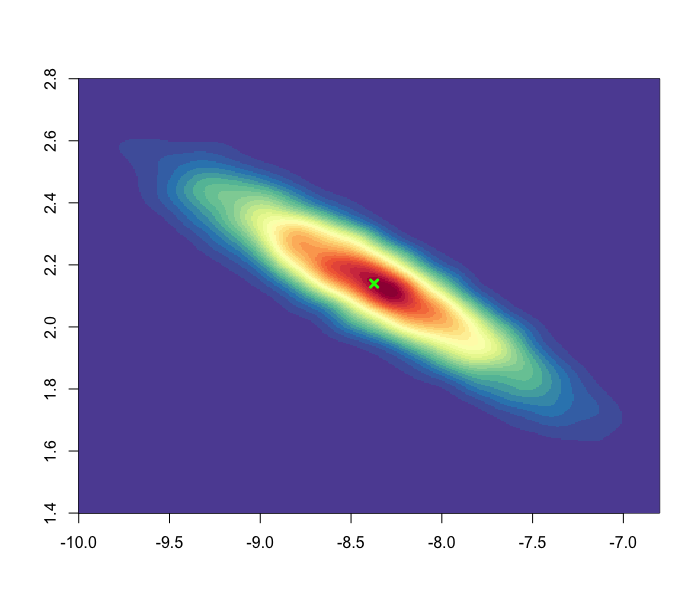
\includegraphics[width=0.6\textwidth]{heatmap-log-linearity-SliceSampling-new-2}
%	\tag{1}
	\caption{Approximated posterior density of the two dimensional log linearity constant of a two dimensional DPP. The MLE estimator is marked green.}
	\label{fig:3.1}
\end{figure}

A second advantage over the MLE presented in the third chapter is, that it might be possible to computationally approximate the posterior density but not the MLE. This is typically the case if the log likelihood function is not concave, like in the setting of the MLE of the whole elementary kernel \(L\). In fact only hard step in the calculation of the posterior \eqref{post} is the computation of the normalisation constant
\[\int f_{X,\Theta}(x, \theta) \nu(\mathrm{d}\theta). \]
This step can actually also not be performed efficiently for the case of the estimation of \(L\), however we will introduce the methods of Markov chain Monte Carlo simulation that allow an approximation of the posterior without the need to compute the normalisation contant.
\end{emp}

\begin{emp}[Regularisation through the prior]

\end{emp}

%\begin{enumerate}
%\item explain general procedure and say something about intuition
%\item explain the benefits, namely:
%\begin{enumerate}
% \item can capture uncertainty
% \item might me more feasible
% \item is an extension, at least if there is a uniform distribution on the parameter space
%\item offers a method for regularisation, i.e. will sometimes work if MLE doesn�t (properly) work due to statistical fluctuations like overfitting of noise
%\end{enumerate}
%\item 
%\end{enumerate}

\section{Markov chain Monte Carlo methods}

\subsection{Reminder on Markov chains}

\begin{enumerate}
\item Definition
\item irreducibility
\item existence of stationary distributions
\item reversibility
\item detail-balance
\item Ergodicity 
\item idea of MCMC
\end{enumerate}

\subsubsection*{Irreducibility and existence of stationary distributions}

\subsubsection*{Ergodicity}

\subsubsection*{Idea of Markov chain Monte Carlo methods}

\subsection{Metropolis-Hastings random walk}

\subsubsection*{Presentation of the model}

\subsubsection*{Acceptance rate, effective sample size and Tuning}

\subsection{Slice sampling}

\subsubsection*{Presentation of the model}

\subsubsection*{Realisation of the model}

%\subsection{Tuning the algorithm}

\section{The variational approach}

%\section{Towards deep DPPs}

%\section{A Bayesian approach to the kernel estimation}